\appendix

%\begin{figure*}[th]
%\centering
%\section*{\hspace{5em}\mytitle: Appendix}
\section*{Appendix}
%\end{figure*}
%\appendix

\section{Further Implementation Details}
\subsection{Scaling Function} \label{ss:sf}
$p^A_{ij}$ has a value range of $[1, N]$, which depends on the size of the input problem instance. Moreover, general deep-learning frameworks (e.g., PyTorch and TensorFlow) initialize model weights under the assumption where the maximum value in the input data is around $1.0$.
Hence, to re-scale $p^A_{ij}$ to $s^A_{ij}$, we used the following function $h$, which is
\begin{equation}
\begin{split}
    h(p^A_{ij}) = ((1-\lowest)(N-p^A_{ij}))/N + \lowest \\
    h(p^B_{ji}) = ((1-\lowest)(N-p^B_{ji}))/N + \lowest, \\
\end{split}
\end{equation}
where $\lowest$ should be a constant value in range $(0,1)$ and is set to 0.1 in our experiments.

%\subsection{Loss to constrain the matrix to be doubly stochastic} \label{ss:lossc}


\subsection{Visualization of Set Encoder and Calculation Cost} \label{ss:set_encoder}
The purpose of the set encoder is to embed the feature of an edge $a_i\rightarrow b_j$ while considering the relative relationship among the other out-edges from $a_i$.
Because the number of out-edges is variable, the set encoder should also accept variable-size inputs.
Besides, since the set of edges have no order, the encoder should output a permutation invariant result.

Such network structure is proposed in \cite{deepset} and \cite{pointnet}. Following these studies, we implemented the encoder of WeaveNet as a structure that has two convolutional layers with a set-wise max-pooling layer. The pooling is done for each element in the feature vector and yields a single vector, which is then concatenated to each input feature. The illustration is in Fig.~\ref{fig:conv_with_global_max_pooling}.
In the experimental part, we refer to the number of output channels from the convolutional layers as $D'$ and $D$, where $D'$ is the intermediate feature fed to the max-pooling layer and $D$ is the output of this encoder. Following \cite{pointnet}, $D'$ is typically set larger than $D$.
Note that the structure is followed by the batch normalization and activation, for which we adopted the PReLU function. 

\subsubsection{Computational Complexity}
With $D_{\max} = \max\{D',D\}$, the theoretical calculation cost of a single set encoder on a single core processing unit is $O(N^2D_{\max}^2)$, where a single linear operation in the convolution requires $D^2$ and we repeat it for $2N\times M$ elements ($N\geq M$).
The other operations in WeaveNet, such as cross-concatenation, clearly have less cost. Hence, the entire WeaveNet has its calculation cost of $O(LN^2D_{\max}^2)$.

We can reduce this into $O(L\log(ND_{\max}))$ with an ideal parallel processing unit.
We have $2N\times M$ elements for the convolution and can linearly operate them independently. Each linear operation can be done in parallel except for weighted sum aggregation, which takes $O(\log(D_{\max}))$. Besides, we have a max-pooling operation, which consists of $D$ parallel max operations. It can also be done in parallel and each max operation for $N$ elements takes $O(\log N)$. Therefore, we can execute the calculation of a single set encoder in $O(\log(N)+\log(D_{\max}))$.


\begin{figure}[ht!]
    \centering
    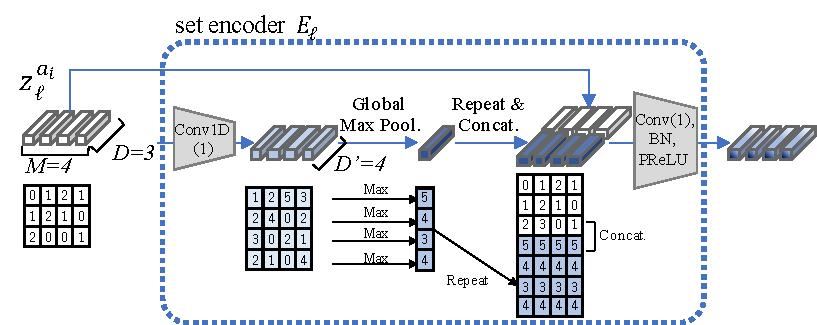
\includegraphics[width=1.0\linewidth]{figures/conv_with_global_max_pooling.pdf}
    \caption{Illustration of the process in set encoder $E_\ell$, where $z_\ell^{a_i}$ (colored in white) is once encoded to $D'$ channel features (colored in pale blue), then max-pooled to obtain statistics in the feature set (colored in blue). The statistics information is concatenated to each input feature and further encoded (color in a gradation).}
    %\jm{This figure is a little confusing to me: in my mind I cannot easily find the correspondence between the 3d block (1xMxD) and the 2d 3x3 grid. I hope there can be explanations about how to do the 3d-2d transfer.}\ah{How about this?}
    \label{fig:conv_with_global_max_pooling}
\end{figure}


\subsection{Information Propagation with WeaveNet}\label{app:scope}
\begin{figure}[t!]
    \centering
    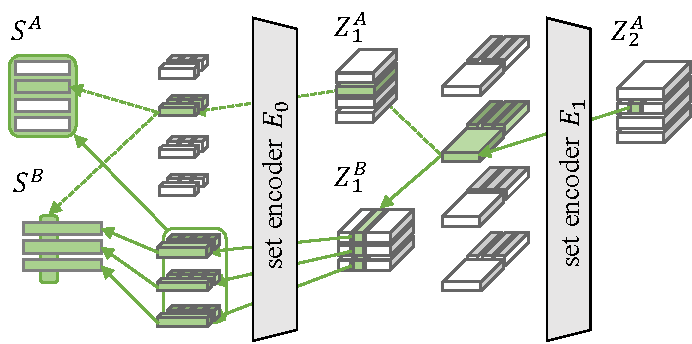
\includegraphics[width=1.0\linewidth]{figures/backward_path.pdf}
    \caption{Backward path of WeaveNet (two-stream architecture) from $ij$-th feature in $Z^A_2$. The upper stream terminates at $i$-th row of $S^A$ and $i$-th column of $S^B$, which are the weights on outgoing and incoming edges of the agent $a_i$, respectively. 
    The lower stream refers to all the elements in $S^A$ and $S^B$.}
    \label{fig:backward_path}
\end{figure}
\begin{figure}[t!]
    \centering
    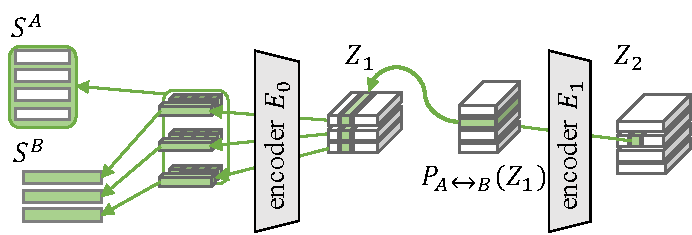
\includegraphics[width=1.0\linewidth]{figures/backward_path_DBM.pdf}
    \caption{Backward path of DBM (single-stream architecture) from $ij$-th feature in $Z_2$, where the stream refers to all the elements in $S^A$ and $S^B$. This structure is common with SSWN.}
    \label{fig:backward_path_dbm}
\end{figure}

\begin{figure*}[!t]
    \centering
    \begin{minipage}{0.5\textwidth}
    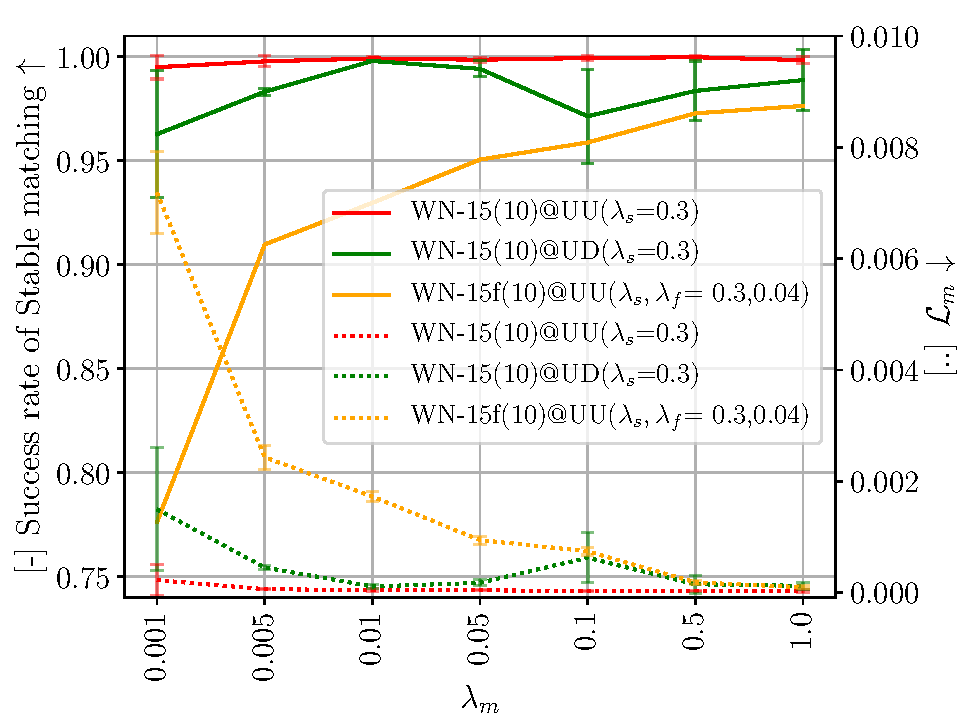
\includegraphics[width=0.9\linewidth]{figures/Fig10.pdf}
    \vspace{-0.5em}
    \caption{Sensitivity against $\lambda_m$}
    \label{fig:suppli_c}
    \end{minipage}%
    \begin{minipage}{0.5\textwidth}
    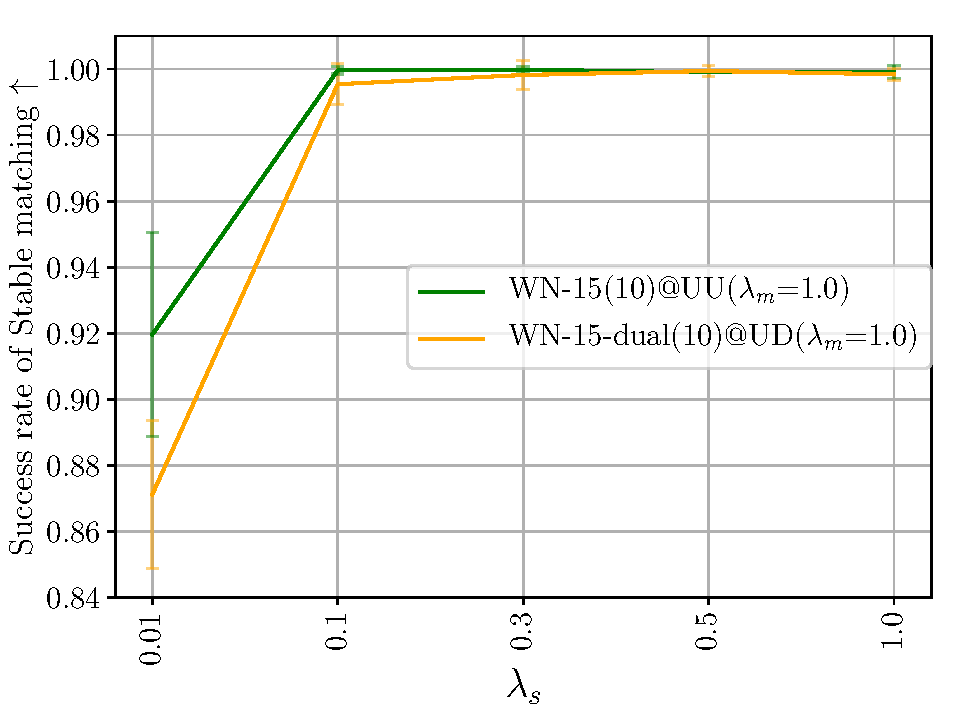
\includegraphics[width=0.9\linewidth]{figures/Fig11.pdf}
    \vspace{-0.5em}
    \caption{Sensitivity against $\lambda_s$}
    \label{fig:suppli_s}
    \end{minipage}\\
    \begin{minipage}{0.5\textwidth}
    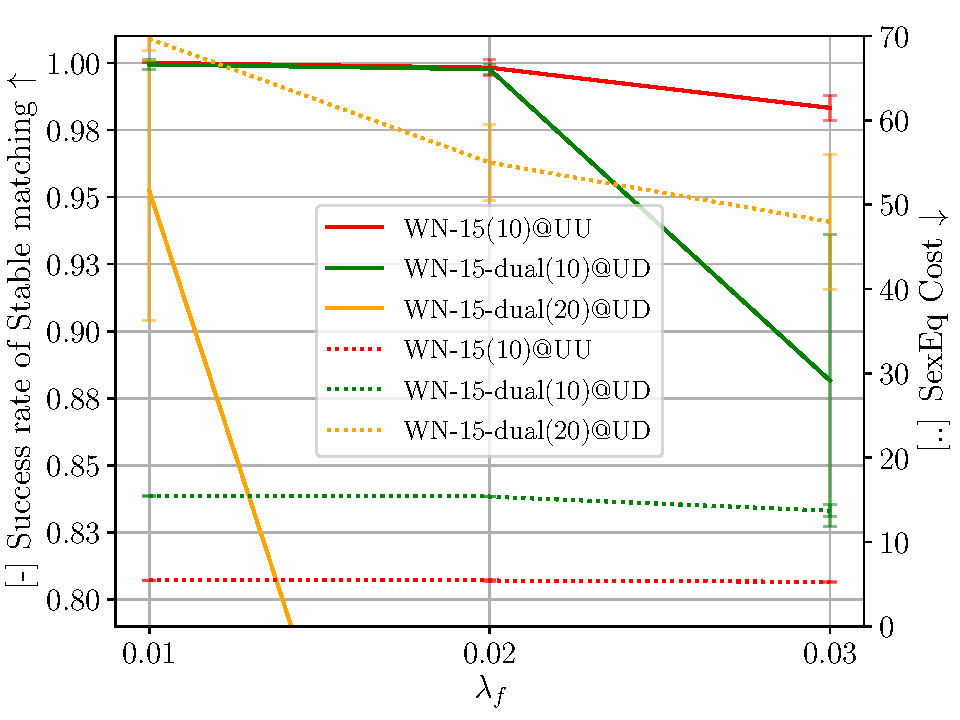
\includegraphics[width=0.9\linewidth]{figures/Fig12.pdf}
    \vspace{-0.5em}
    \caption{Sensitivity against $\lambda_f$}
    \label{fig:suppli_f}
    \end{minipage}%
    \begin{minipage}{0.5\textwidth}
    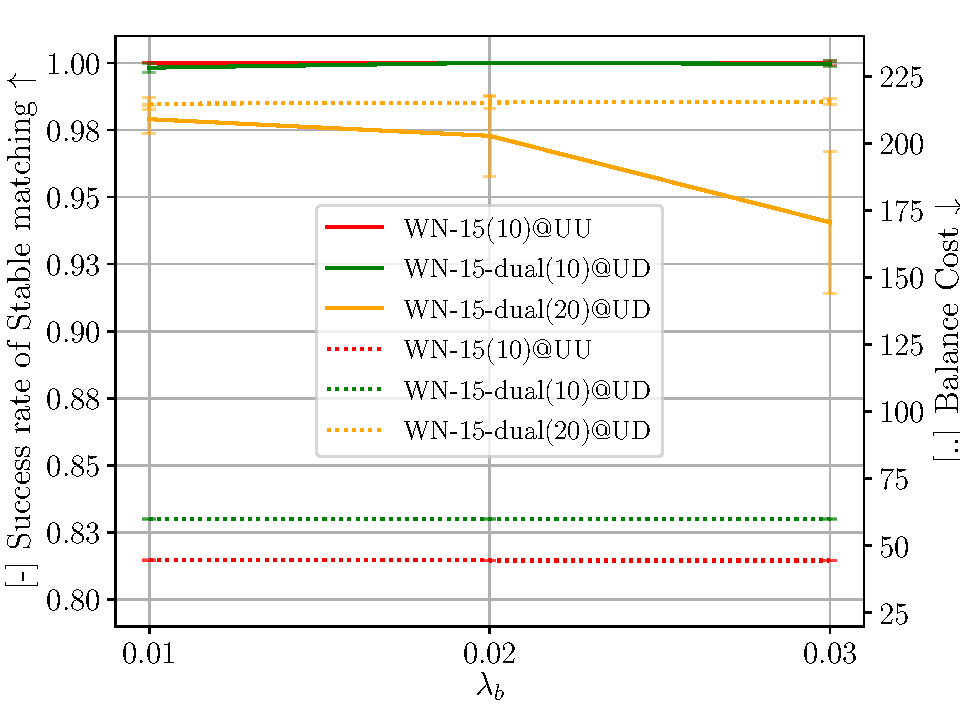
\includegraphics[width=0.9\linewidth]{figures/Fig13.pdf}
    \vspace{-0.5em}
    \caption{Sensitivity against $\lambda_b$}
    \label{fig:suppli_b}
    \end{minipage}
\end{figure*}

\checkedby{Jiaxin}{Hashi}
By stacking two or more FW layers, every latent feature of $ij$-th element in $Z^*_\ell$ ($\ell\geq 2$) has a receptive field that covers all over the preference lists.
Fig.~\ref{fig:backward_path} illustrates the receptive field, where green elements are upstream components of the $ij$-th element, and $E_0$, $E_1$ are encoders that involve all the input into the calculation of each feature in the output sequence. 
Let us backtrack the path of back-propagation from the $ij$-th element in $Z^A_2$.
It derives from the $i$-th row of $Z^A_1$ and the $i$-th column of $Z^B_1$.
Focusing on the $i$-th column (e.g., the green column) of $Z^B_1$, each element (in the $k$-th row) derives from all the elements in the $k$-th row of $S^B$, plus all the elements in the $k$-th column of $S^A$.
In this way, all the elements in $S^A$ and $S^B$ contribute to a column of $Z^B_1$, then an element of $Z^A_2$.
Symmetrically, all the elements in $S^A$ and $S^B$ contribute to a column of $Z^A_1$, then an element of $Z^B_2$.
Hence, we can see that stacking two FW layers can cover the entire bipartite graph in its reference.
% because the diameter of a complete bipartite graph is always two.




We also visualize the back-propagation path of DBM in Fig.~\ref{fig:backward_path_dbm}.
DBM also covers the entire bipartite graph within two layers, but each encoder is used only for one direction (either weftwise or warpwise). Here, the path in Fig.~\ref{fig:backward_path_dbm} is identical with the lower path in Fig.~\ref{fig:backward_path}. From this perspective, WeaveNet innately contains the path of DBM.
%We can also see that the feature from the upper path always derives from the edges connected to an agent while the lower path from the entire graph. Hence, this structure explicitly assigns the former $D$ dimensions of the input of the set encoder to be more agent-specific while the latter $D$ dimensions to be more graph-specific. In other words, the structure encourages the encoder to contrast these two components, which would facilitate a good convergence.

\subsection{Loss Weights}\label{app:hyperparameters}


Through the experiments, we set the loss weights $\lambda_m=1.0$, $\lambda_s=0.7$, and $\lambda_f=\lambda_b=0.01$ to train any learning-based methods.
We adjusted these parameters in the following process.

As a preliminary model, we prepared WN-15 with a set encoder with $D=64$ and $D'=256$. In this investigation, we used a balanced dataset UU and the most biased dataset UD.

Because we experimentally found the tendency that the model hardly outputs a stably matched solution without minimizing $\loss_m$, we first tried to fix $\loss_m$.
Fig.~\ref{fig:suppli_c} shows the success rate of stable matching with different $\loss_m$ in the range $\{0.001,~0.005,~0.010,~0.050,~0.100,~0.500,~1.000\}$, where WN-15($n$) is the model trained and validated with the samples of $N=n$. 
From this result, we decided to set $\lambda_m=1.0$ and use it as the maximum weight among the loss weights.

Next, fixing $\lambda_m=1.0$, we observed the trend in success rate of stable matching against $\lambda_s$. Fig.~\ref{fig:suppli_s} shows our investigation of $\loss_s$ in the range $\{0.01,0.10,0.30,0.50,1.00\}$. 
Here, WN-dual is a WeaveNet variant to deal with the inconsistent distributions of UD (see \ref{ss:exp2_supp} for details of WN-dual).
As a result, we found that $\lambda_s$ should simply be large enough (ca. $\lambda_s\geq 0.30$).

To investigate sensitivity of the model against $\lambda_f$ and $\lambda_b$, in this experiment, we set $\lambda_s=0.3$ as the minimum satisfiable value in Fig.~\ref{fig:suppli_s}\footnote{We used $\lambda_s=0.7$ in any other experiments to stabilize the results, as stated in Section \ref{s:exp}.}, and obtained Figures \ref{fig:suppli_f} and \ref{fig:suppli_b}. From these figures, we found that too-strong weights for fairness may disrupt stability, which matches a theoretical expectation. Hence, we decided to use $\lambda_f=\lambda_b=0.01$, which achieved the highest success rate of stable matching in the search range of $\{0.01,0.02,0.03\}$.

\begin{comment}
WeaveNetのFW層(図\ref{fig:feature_weaving_layer})の
横糸成分$Z^A_{\ell}$と縦糸成分$Z^B_{\ell}$の次元数$D$は,
{8,16,32,64}から64を選択した.
Feature weaving layer内のadjacent-edge-encoder $E_l$(図\ref{fig:conv_with_global_max_pooling})内
で使われる特徴ベクトルの次元数は,$Z^A_{\ell}$,$Z^B_{\ell}$ の{4,8,16,32}から32を選択した.
learning rate($lr$)は, 探索的に0.0001を選択した.
これらは,agentサイズ$20 \times 20$ $\lambda_s = 0.7$, $\lambda_m = 1$の条件下で決定された.

本論文の表\ref{tab:weave_net_variations}で使われた
WN\eqref{eq:lsm}, WNf\eqref{eq:lfsm}, WNb\eqref{eq:lbsm}
のHyper parameters, $\lambda_m$, $\lambda_s$, $\lambda_f$, $\lambda_b$の決定方法について示す.
図\ref{fig:suppli_c}は, $\lambda_s$を0.7に固定した条件で, $\lambda_m$を変えたときのStability matching rateと$\loss_m$の変化である．
入力分布としてAgent size 20のUUとし, モデルとして 
$\lambda_f = 0.01$としたWNf\eqref{eq:lfsm}を用いた.
結果として$\lambda_m$を1に近づけると$\loss_m$は, 0に漸近し, stability matching rate が1に近づくことから, $\lambda_m = 1$を採用した.
%\sone{再計算 20x20 UU(64,64)-L60 1万回　$\lambda_m = \{0.125,0.25,0.5,1\} $}

図\ref{fig:suppli_c}は, $\lambda_m = 1$に固定した条件で, $\lambda_s$を変えたときのStability matching rateの変化である．
$\lambda_s \ge 0.7 $からStability matching rateが1に漸近する結果を踏まえて
$\lambda_s = 0.7 $とした.
%\sone{再計算 20x20 UU(64,64)-L60 1万回　$\lambda_s = \{0.3,0.5,0.7,1.0 \} $}

図\ref{fig:suppli_f}は, $\lambda_m = 1, \lambda_s = 0.7$に固定した条件で, $\lambda_f$を変えたときのStability matching rateとSexEq Costの変化である．
入力分布としてAgent size 20のUDaとした.
$\lambda_f \ge 0.01 $からStability matching rateは特に20x20 UDにおいて顕著に
悪化し,SexEq Costも減少していったことから$\lambda_f = 0.01 $とした.
%\sone{再計算 20x20 UD(64,64)-L60 1万回　$\lambda_f = \{0.01,0.02,0.03\} $}

\end{comment}
%図\ref{fig:suppli_b}は, $lambda_c = 1, \lambda_s = 0.3$に固定した条件で, %$\lambda_b$を変えたときのStability matching rateとBalance Costの変化である．
%入力分布としてAgent size 10のUU, Agent size 20のUU,UDとした.
%$\lambda_b = 0.01 $の時点ですでにStability matching rateは,20x20 UDにおいて0.98ほど落ちており, %$\lambda_b \ge 0.01 $になると急激に
%Stability maching rateは悪化したため, $\lambda_b = 0.01 $を採用した.
%\sone{再計算 20x20 UD(64,64)-L60 1万回　$\lambda_sf = \{0.01,0.02,0.03\} $}
   


%%%%%%%%%%
\subsection{Network Architecture}\label{ss:archi}
%%%%%%%%%%
We can customize the shape of WeaveNet architecture finely by using set encoders with different shapes in each FW layer; however, we avoided such a complex architecture design to simplify the analysis and decided to use common-shape set encoders for all $L$ FW layers.
With this setting, we have only three hyper-parameters to decide the architecture: $L$, $D$, and $D'$. The shortcut path is regularly connected to the input of $\ell$-th layer with an even number of $\ell$.

\begin{table}[ht]
    \centering
{    \small
     \setlength\tabcolsep{2pt} % セルの左右の余白
    \begin{tabular}{lrrrrr}
    \toprule
        \multicolumn{1}{c}{Name} & \multicolumn{1}{c}{$L$} & \multicolumn{1}{c}{$D$} & \multicolumn{1}{c}{$D'$} & \multicolumn{1}{c}{\# of params.} & \multicolumn{1}{c}{Stably Matched (\%)} \\
        \midrule
        Deep  & 30 & 22 & 44 & 117k & 95.7\% \\  %116,736
        Wide1 & 15 & 32 & 64 & 119k & 76.0\% \\ %119,396
        Wide2 & 15 & 24 & 98 & 120k & 73.1\% \\ %120,110
        \bottomrule
    \end{tabular}
}
    \caption{Comparison in parameter efficiency among different shape architectures. Deep achieved the best success rate in stable matching despite its smallest architecture.}
    \label{tab:supp_architecture}
\end{table} 

Table \ref{tab:supp_architecture} shows the success rate of stable matching after 100,000 iterations of training. Here, we drew samples from the UU distribution with $N=30$ for both training and validation.
The result shows that the deepest model performs the best despite its smallest number of parameters. Hence, we decided to use the set encoder that has $D\leq 32$ and $D'=2D$.

\begin{figure}[ht]
    \centering
    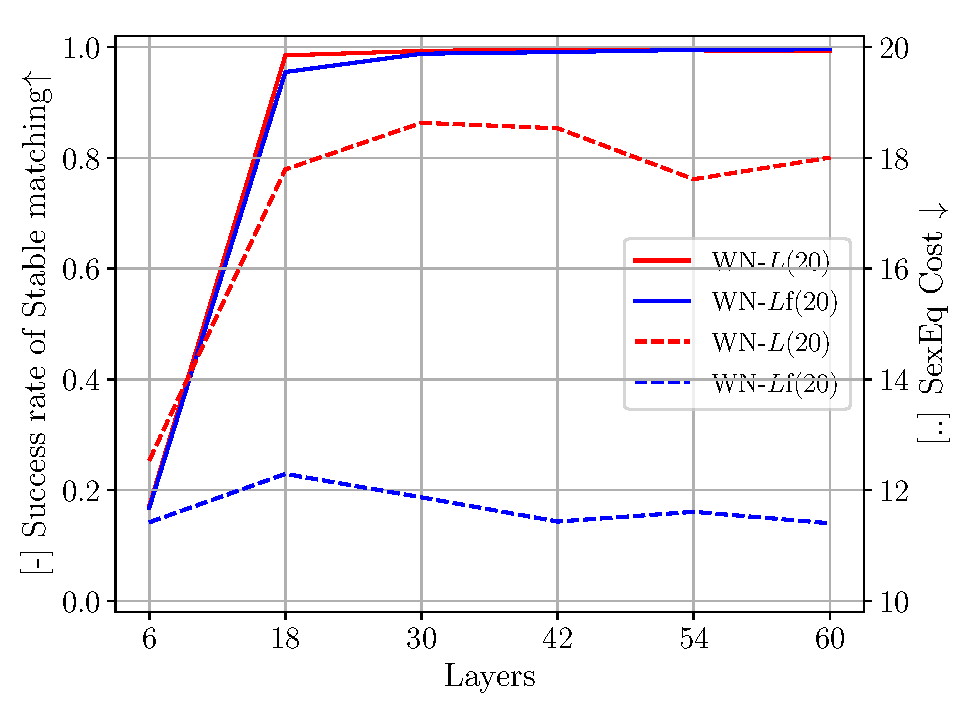
\includegraphics[width=1.0\linewidth]{figures/Fig14_sm.pdf}
    \caption{Success rate of stable matching (solid, $\uparrow$) and $\SEq$ (dashed, $\downarrow$) according to $L$.}
%この図は，横軸が$L$で縦軸がsuccess rate of stable matchingの図に置き換えられる予定．\url{https://gitlab.com/sinicx/interaction/qanda-social-app/-/issues/74}の4.
    \label{fig:impact_of_depth}
\end{figure}

We further investigated the impact of network depth on the problem.
To observe how the strongly NP-hard target increases the difficulty in optimization, we plotted both results by WN-$L$ and WN-$L$f with $L\in \{6,18,30,42,54,60\}$. 
Fig.~\ref{fig:impact_of_depth} shows the trend of success rate against different $L$. Here, the models were trained and validated with the UU dataset at $N=20$.
We can see from the result that $L=6$ is not enough to stably match samples of $N=20$, but $L=18$ is enough if only for that purpose.
Besides, we observed that a deeper stack of layers tends to improve $\SEq$ slightly.
% task 


\begin{comment}
\section{Hyper-parameter Settings} \label{ss:weaveNetPara}
\begin{table}[ht]
  \centering
    \caption{WeaveNet parameter} 
		\begin{tabular}{l|r}
		\midrule \midrule
		Parameters & Optimal value  \\ \midrule 
		FWL & 60  \\
		FWL node dimension  & 32 \\
		set encoder node dimension & 64  \\
		$lr$ Larning rate & 0.0001 \\ %←これはArchitecture???
		\midrule
		\end{tabular}
		\label{table:weavenetpara}
  \hfill
\end{table}

%この論文で提案されたWeaveNetの4つのHyper parameterは, 
%探索的に求め, Stability matching rateが一番良かったパラメータを採用した.　
%採用したパラメータの一覧を表\ref{table:weavenetpara}に示す.
%WeaveNetのFeature Weaving Layers(FWL,図\ref{fig:weavenet})は,
%{6,18,30,42,54,60}から60を選択した.
%\sone{計算した 20x20 UU(64,64)-L?? 2万回} 
\end{comment}



\begin{table}[!ht]
    \centering
     \setlength\tabcolsep{4pt} % セルの左右の余白
    {\small
    \begin{tabular}{lrrrrr}
    \toprule
        \multicolumn{1}{c}{Model} & \multicolumn{1}{c}{Encoder} &  \multicolumn{1}{c}{$D$} & \multicolumn{1}{c}{$D'$} & Res. &\# of params. \\
        \midrule
        MLP-3  & dense layer & 100 & - & w/o & 28k  \\ % 28475
        GIN-2 & graph conv. & 44 & - & w/o & 29k \\ %
        DBM-6 & max pooling & 48 & - & w/o & 29k  \\ % 28809
        DBM\_A-6 & self-attention & 48 & 32 & w/ & 28k\\ %
        SSWN-6 & set encoder  & 48 & 48 & w/o & 25k \\ % 25108
        SSWN-60 & set encoder & 64 & 64 & w/ & 740k \\ %740932
        %SSWN-12 & set encoder & 24 & 24 & w/ & 21k \\ % 20572
        WN-6 & set encoder & 24 & 48 & w/o & 25k \\ % 24964
        WN\_A-6 & self-attention & 32 & 28 & w/ & 29k \\ %
        WN-18 & set encoder & 32 & 64 & w/ & 143k \\ %143876
        WN-60 & set encoder & 32 & 64 & w/ & 493k \\ %
        WN-80 & set encoder & 32 & 64 & w/ & 659k \\
        \bottomrule
    \end{tabular}
    }
    \caption{Hyper-parameters for each baseline, where $D'$ represents the length of key and query features for self-attention, and the max-pooling input for the set encoder. Note that the $D$-dimentional feature of WN is cross-concatenated and processed as a $2D$-dimensional features in the encoders. }\label{tab:hypara_baselines}
    %\ah{SSWN-12って外すことにしてませんでした？記憶が怪しいが．}\sone{SSWN-12 外します}
\end{table} 

\subsection{Hyper-parameter Settings for the Other Baselines}\label{ss:supp_hypara_baseline}

Here, we denote the hyper-parameters for learning-based baseline methods, including those used in \ref{ss:exp1_supp} and \ref{ss:exp2_supp}. 
The detail is summarized in Table \ref{tab:hypara_baselines}. Note that MLP could not converge when more than three hidden layers are stacked. Hence, we set the number of layers to be three, as used in \cite{harvard2019}. For GIN \cite{xu2018how}, we put two layers because the original paper reported it performs best. Besides that, some papers provide theoretical analyses that graph convolutional networks (GCNs) suffer from over-smoothing \cite{li2018deeper,Oono2020Graph}. Namely, it loses the discriminative capacity for nodes on a dense graph when the layers are deeply stacked. This is exactly our case because a complete bipartite graph is always dense; its connection density is $N/(2N-1)(>1/2)$ (there are $2N^2$ edges among $2N(2N-1)$ possible edges). Hence, a deeper stack does not contribute to solving the problem.


Note that we used the same loss weights decided in \ref{app:hyperparameters} for all the methods since the loss weights derive from the task property rather than the architecture.
For simplicity in comparison, we also used the three hyper-parameters, $L$, $D$, and $D'$, to identify the architecture following to \ref{ss:archi}. We experimentally decided whether to use the residual structure or not for the models which have more than four layers. Hence, the shown results are always better ones.





\section{Additional Experiments}\label{ss:supp_additional_exp}
\subsection{Additional Learning-based Baselines and Ablations.}\label{ss:exp1_supp}

%\subsubsection{Baselines and an Ablation}
\begin{figure}[th]
    \centering
    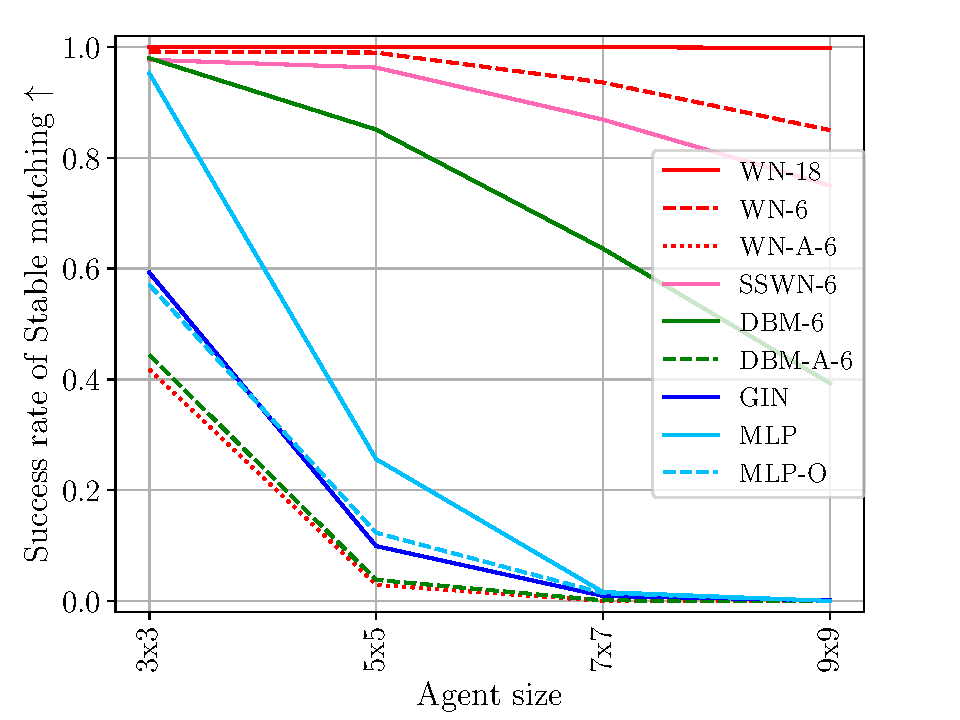
\includegraphics[width=1.0\linewidth]{figures/Fig15_sm.pdf}
    \caption{Change in success rate of stable matching ($\uparrow$) according to $N$, as a complement of Fig.~\ref{fig:Ex1_a}.}
    \label{fig:exp1_supp}
\end{figure}

We compared WeaveNet to more comprehensive baselines: a variation of MLP, DBM, WeaveNet, and a GCN model.
Fig.~\ref{fig:exp1_supp} shows the results.

{\bf MLP-O} is a variant of MLP that faithfully follows the loss functions proposed in \cite{harvard2019}.
The difference is in the matrix constraint loss function $\loss_m$.
Ours defined in Eq.~\eqref{eq:loss_c_p2} is cosine-distance based, while the one proposed in the original paper is Euclidean-distance based, which is
\begin{equation}
\begin{split}
\loss_m(\hat{m}^A,\hat{m}^B) & = \sum_{\{i,j\}\in A\times B} |\hat{m}^A_{ij} - \hat{m}^B_{ji} |.
\end{split}
\label{eq:loss_c_orig}
\end{equation}

The above loss function restricts $i$-th column and $i$-th row of $\hat{m}$ to be the same point in the $N\times M$ space. In other words, the column and row must match in a scale variant manner.
We considered that this is unnecessarily strict for maintaining $\hat{m}$ to be symmetric. Hence we adopted the cosine distance for $\loss_m$. 
In Fig.~\ref{fig:exp1_supp}, we observed that MLP has a clear performance gain from MLP-O by our cosine-distance-based $\loss_m$.

{\bf GIN} is the state-of-the-art GCN architecture \cite{xu2018how}.
Some readers may consider GCNs as the solution to this problem. 
We put two GIN layers followed by one Linear layer that outputs $\hat{m}$ as a flat vector as MLP. From the result, we confirmed that the GCN is not suitable to solve this problem.

DBM proposed in \cite{gibbons2019deep} has two variations; one uses max-pooling with one convolutional layer\footnote{The max-pooled feature is copied and concatenated to the input feature as the set encoder, but it does not have convolution before the max-pooling operation.} as the layer-wise encoder (DBM) and self-attention (DBM\_A). 
We also integrated self-attention into the WeaveNet architecture ({\bf WN\_A-6}) to complete the comparison of the encoder choice. 
As a result, we have confirmed that self-attention does not work well for stable matching problem.


\begin{table*}[th!]
\setul{1pt}{.4pt}
\centering
{\small

\begin{tabular}{lrrrrr|rrrrr}
\toprule
Agents ($N\times M$) & \multicolumn{5}{c|}{20$\times$20}  & \multicolumn{5}{c}{30$\times$30}  \\ \midrule
      Datasets (Distribution Type)     & \multicolumn{1}{c}{UU}    & \multicolumn{1}{c}{DD}    & \multicolumn{1}{c}{GG}    & \multicolumn{1}{c}{UD}     & \multicolumn{1}{c}{Lib}    & \multicolumn{1}{|c}{UU}    & \multicolumn{1}{c}{DD}    & \multicolumn{1}{c}{GG}    & \multicolumn{1}{c}{UD}     & \multicolumn{1}{c}{Lib} \\ \midrule
WN-60f-sym             & \ul{11.44}  & \ul{6.32} &  \ul{15.34} & 81.21 & 14.39 & \ul{16.07} & \ul{9.64}  & \ul{26.46} & 194.24  & 21.16 \\
Stably Matched (\%)  & \ul{99.10} & \ul{99.40}  & \ul{99.40} & 96.00  & 99.50 & \ul{98.10}  & \ul{99.00}  & \ul{98.00} & 81.50  & 98.80 \\ \midrule
WN-60f-asym          & -& -& -& \ul{71.18} & \ul{14.44} & -& -& -& \ul{162.61} & \ul{21.29} \\
Stably Matched (\%)  & -& -& -& \ul{99.50} & \ul{99.80} & -& -& -& \ul{93.90} & \ul{98.60}\\ \midrule
WN-60f-dual          & -& -& -& 71.25 & 14.58 & - & - & - & 163.71 & 22.12\\
Stably Matched (\%)  & -& -& -& 98.50 & 99.60 & - & - & - & 94.80  & 97.50 \\ \midrule
WN-60f(20)          & 11.49 & 6.20 & 15.30 & 71.10 & 14.40 & 16.66 & 9.55 & 26.57 & 162.91 &  21.82 \\
Stably Matched (\%) & 98.90 & 99.50 & 99.40 & 99.60 & 99.30 & 94.60 & 97.30 & 95.70 & 91.30 & 97.70 \\ \midrule
SSWN-60f          &  12.82 & 7.41 & 16.62 & 70.94 & 15.20 & 19.13 & 12.76 & 28.33 & 160.83 & 22.45 \\
Stably Matched (\%)  & 95.80 & 99.20 & 96.50 & 92.40 & 97.90 & 90.00 & 97.50 & 89.00 & 69.20 & 92.30  \\ \midrule \midrule
WN-60f+Hung &   11.51 &	6.35 & 15.37 &	71.18 &	14.45 &	16.14 &	9.69 & 26.58 & 	162.73 & 21.32  \\ 
Stably Matched (\%)  &  99.80 & 99.90 & 100.00 & 99.60 & 100.00 & 99.70 & 99.90 & 99.90 & 95.20 & 99.20 \\ \bottomrule
\end{tabular}
}
\caption{Ablation study for the network architecture difference with $\SEq$ ($\downarrow$) and the success rate of stable matching ($\uparrow$). The scores shown in Table \ref{table:SEqCost} are underlined.}
\end{table*}


\begin{table*}[th!]
\setul{1pt}{.4pt}
\centering
  {\small

\begin{tabular}{lrrrrr|rrrrr}
\toprule
Agents ($N\times M$) & \multicolumn{5}{c|}{20$\times$20}  & \multicolumn{5}{c}{30$\times$30}  \\ \midrule
Datasets (Distribution Type) & \multicolumn{1}{c}{UU}    & \multicolumn{1}{c}{DD}    & \multicolumn{1}{c}{GG}    & \multicolumn{1}{c}{UD}     & \multicolumn{1}{c}{Lib}    & \multicolumn{1}{|c}{UU}    & \multicolumn{1}{c}{DD}    & \multicolumn{1}{c}{GG}    & \multicolumn{1}{c}{UD}     & \multicolumn{1}{c}{Lib} \\ \midrule
WN-60b-sym              & \ul{71.29} & \ul{138.57} & \ul{106.50} & 141.96 & 65.59 & \ul{137.70} & \ul{301.08} & \ul{221.12} & 315.51 & 127.05 \\
Stably Matched (\%)     & \ul{98.00} & \ul{99.10}  & \ul{98.60}  & 97.30  & 98.90 & \ul{97.90}  & \ul{98.60}  & \ul{93.70}  & 80.30  & 98.10 \\ \midrule
WN-60b-asym          & -& -& -& \ul{140.72} & \ul{65.63} & -& -& -& \ul{313.11} & \ul{127.12} \\
Stably Matched (\%)  & -& -& -& \ul{99.80} & \ul{99.10} & -& -& -& \ul{98.80} & \ul{98.00}\\ \midrule
WN-60b-dual          & -& -& -& 141.20 & 65.70 & - & - & - & 314.79 & 127.25 \\
Stably Matched (\%)  & -& -& -& 99.60 & 99.30 & - & - & - & 98.90 & 97.90 \\ \midrule
WN-60b(20)          & 71.05 & 138.53 & 106.13 & 140.81 & 65.53 & 137.06 & 301.21 & 220.23 & 313.68 & 127.62 \\
Stably Matched (\%)  & 98.50 & 98.80 & 99.50 & 99.70  & 98.80 & 96.10 & 96.70 & 95.00 & 88.90 & 93.80 \\ \midrule
SSWN-60b             & 76.54 & 139.29 & 107.58 & 141.37 & 66.99 & 150.88 & 302.90 & 223.62 & 314.91 & 129.52 \\
Stably Matched (\%)  & 92.60 & 98.50 & 98.40 &  99.60 & 98.60 & 79.80 & 96.70 & 93.90 & 94.0 & 92.80 \\ \midrule \midrule
WN-60b+Hung & 71.45 & 138.60 & 106.55 & 140.73 & 65.68 & 137.92 & 301.14 & 221.42 & 313.13 & 127.22 \\ 
Stably Matched (\%)  & 99.90 & 99.90 & 99.60 & 99.90 & 100.00 & 99.00 & 99.90 & 96.90 & 99.30 & 99.20 \\ \bottomrule
\end{tabular}
}
\caption{Ablation study for the network architecture difference with $Bal$ ($\downarrow$) and the success rate of stable matching ($\uparrow$). The scores shown in Table \ref{table:BalCost} are underlined.}
\end{table*}

\subsection{Additional Ablation in \texorpdfstring{$N=20,~30$}{N=20, 30}} 
\label{ss:exp2_supp}

We provide a detailed ablation study to finely analyze the symmetric and asymmetric variants, the effect of two-stream architecture, the size of training samples, and the binarization operation.

First, we refer to the symmetric and asymmetric variants of WN-60f/b as {\bf WN-60f/b-sym} and {\bf WN-60f/b-asym}, respectively. Note that both models have the two-stream architecture, but {\bf sym} shared batch normalization layers and {\bf asym} does not. In addition, {\bf asym} has an additional channel in inputs for side-identifiable code. 
In addition to them, we further prepared {\bf WN-60f/b-dual}, a model that separately holds the entire set encoder for $Z^A_\ell$ and $Z^B_\ell$ at each layer to deal with asymmetric inputs. 
%\ah{ToDo: 全部揃ったら考察を書く．}\sone{全部そろった！}\ah{書いた!}
Since UD is a highly asymmetric dataset, the symmetric variant (WN-60f/b-sym) does not work appropriately while the asymmetric variants ({\it asym} and {\it dual}) could deal with it.
In the dataset Lib, where we assumed an unknown bias strength, {\it asym} worked as well as {\it sym} and {\it dual}. This result showed that we can safely apply the asymmetric variation for any situation.

Comparing {\it asym} with {\it dual}, {\it asym} marked slightly smaller fairness costs than {\it dual} while keeping comparative success rate in stable matching.
This result experimentally confirmed the parameter efficiency of {\it asym} against {\it dual} since {\it dual} has roughly twice more parameters than {\it asym}.

Second, to investigate the effect of choosing different training sample size, we prepared {\bf WN-60f/b(20)}, a model trained by samples of $N=20$, and applied it to test datasets of $N=20,~30$. The asymmetric variant was applied for UD and Lib.
From the results, we confirmed that the models trained with $N=30$ has no degradation from WN-60f/b(20) even when tested at $N=20$. In contrast, WN-60f/b(20) did not perform well when applied to the samples of $N=30$.
This trend implies that we should train the model with a larger $N$ to cover a wide range of input-size variations.

Third, {\bf SSWN-60}, a single-stream WeaveNet with set encoders, was prepared to measure the contribution of the two-stream architecture. 
SSWN-60f/b achieved consistently worse result than WN-60f/b (underlined), and collapsed in UD ($N=30$) in Table~\ref{table:SEqCost} and UU ($N=30$) in Table~\ref{table:BalCost}.
These results experimentally proved the importance of the two-stream structure.

Finally, to avoid an increase of theoretical calculation cost, WeaveNet applied ${\rm argmax}$ operation to binarize $\hat{m}$ rather than the Hungarian algorithm, whose calculation cost is $O(N^3)$. 
To demonstrate how well the network maintains ${\rm argmax}(\hat{m})$ to be a matching, we compared the result with those obtained with the Hungarian algorithm ({\bf WN-60f+Hung}). Again, the asymmetric variant was applied for UD and Lib.
From the result, we confirmed that WN-60f/b+Hung achieved higher success rates in stable matching while worse $\SEq$ and $Bal$ costs. 
This behavior implies that the output matched only by the Hungarian algorithm tends to have higher fairness costs.

To obtain further insight, we prepared Table~\ref{tab:N100_bp}, which summarizes the difference w/ and w/o the Hungarian algorithm at $N=100$. In this setting, we have more samples with which WN-80f/b fails to even obtain one-to-one matching by the ${\rm argmax}$ binarization.
Binarization by the Hungarian algorithm forces such failure estimation $\hat{m}$ to be a matching; however we obtained only 5.0\% additional stable matchings from the 13.4\% failure cases with WN-80f, and 7.5\% from 19.8\% failure cases with WN-80b. A similar number of cases resulted in matchings with more than three blocking pairs. 

From these results, we concluded that the Hungarian algorithm does not essentially improve the quality of fair stable matching, although it ensures $\hat{m}$ to be a one-to-one matching.

\begin{table}
\centering
{    \small
     \setlength\tabcolsep{4pt} % セルの左右の余白
    \begin{tabular}{rrr|rr}
    \toprule
        \multicolumn{1}{c}{\#Block. Pairs} & \multicolumn{1}{c}{WN-80f} & \multicolumn{1}{c|}{+Hung.} & \multicolumn{1}{c}{WN-80b} & \multicolumn{1}{c}{+Hung.} \\
        \midrule
        0  & 84.4\% & 89.4\%     & 73.2\% & 80.8\% \\  %116,736
        1 & 2.2\% & 4.6\%        & 6.7\% & 10.9\% \\ %119,396
        2 & 0.0\% & 0.4\%        & 0.3\% & 1.2\% \\ %120,110
        $\geq 3$ & 0.0\% & 5.6\% & 0.0\% & 7.1\% \\ %120,110
        Fail & 13.4\% & -        & 19.8\% & - \\ %120,110
        \bottomrule
    \end{tabular}
}
    \caption{Number of blocking pairs in the estimated matching with UU $N=100$. Fail counts outputs that are not a one-to-one matching. Outputs with no blocking pairs are stable matchings.}
    \label{tab:N100_bp}
\end{table}

\begin{comment}
\section{Comparison with Graph Convolutional Networks}
It is natural that some readers consider graph convolutional networks (GCNs) as the solution for this problem. However, we could not get any meaningful results with it. Thus we abbreviated to compare any GCN with WeaveNet in the main paper.

To make it reproducible, we describe an example of GCN implementation, whose code will be also included as supplementary material.
As a node feature, we used the preference list of each agent.
The features were input to two stacked GIN layers \cite{xu2018how}. Then their output agent features were concatenated pair-wisely and obtain $N\times M$ pair-wise features. They are input to a common binary estimator as WeaveNet does at Conv(1$\times$1) in Fig.~\ref{fig:weavenet}. Finally, the output of this binary estimator was treated as $\hat{m}$.

The above implementation outputs almost random results.
We consider the reason as follows; GCNs suffer from over-smoothing when graph convolution layers are stacked deeply \cite{li2018deeper,Oono2020Graph}.
%The over-smoothed features lose edge weight information and can represent only edge presence, which is common among the nodes in each group. 
%The diameter of the bipartite graph is only two. This means that more than two stacked layers do not bring any new information but smoothing node feature more and more with dense adjacency relationship.
This would be critical when solving an matching problem because the problem requests a model to differentiate edges and decide a hard matching even when they are quite similar.

WeaveNet avoids the over-smoothing problem by embedding edges, which represent unique node pairs while differentiating the latent feature of such unique pairs by the adjacent-edge-encoder instead of the weighted averaging operation of graph convolution. More simply, WeaveNet held features edge-wisely rather than note-wisely. This made the weighted-averaging operation unnecessary to forward the layered calculation.
\end{comment}

\section{Data for Reproduction}

\subsection{Calculation Time and Computing Infrastructure}
We trained and tested the learning-based models used in the experiments on a single GPU (Tesla V100, memory size 16GB) mounted on NVIDIA DGX-1. We developed the environment on Ubuntu18.04. %You should not remove this description for reproducibility checklist.
\begin{table}
    \centering
  {\small
    \begin{tabular}{lrr}
    \toprule
        \multicolumn{1}{c}{Elapsed Time} & \multicolumn{1}{c}{for training}  & \multicolumn{1}{c}{for test} \\
        & 200,000 iters. & 1,000 samples \\
        \midrule
        WN-6~ ($N=10$)  & 10.39 hours & 5.82 s \\ 
        WN-18 ($N=10$) & 13.10 hours & 14.83 s \\ 
        WN-60 ($N=20$) & 30.10 hours & 75.15 s \\
        WN-60 ($N=30$) & 43.58 hours & 74.10 s \\ 
        WN-80 ($N=100$) & 111.10 hours & 103.66 s \\ 
    \end{tabular}
    }
    \caption{Elapsed time for training and testing the models.}
    \label{tab:elapsed_time}
    % \ah{Reproducibility checklist案件なので必要．}\sone{1000samplesにかかる時間を追記しました}}
\end{table} 

The above training required less than 16GB of memory space in our setting as long as the batch size is no larger than $8$.
The training and inference time are summarized in Table \ref{tab:elapsed_time}.

\subsection{Dataset}
%(reproducibility check list案件なので，絶対に消してはだめ)．
We implemented the data generator for UU, DD, GG, UD, and Lib following the explanation in \cite{tziavelis2019equitable} since they are not provided by the authors. 
In the process, we also extracted the distribution of the LibimSeTi dataset \cite{brozovsky07recommender}, where the original data of the LibimSeTi dataset is accessible in \url{http://www.occamslab.com/petricek/data/}. 
We filtered out data that do not have bidirectional preference rank, as stated in \cite{tziavelis2019equitable}.
We yielded the validation and test datasets with a fixed random seed to make them reproducible. 

All the code for data generation is included in the submission (with the random seeds and fairness costs of each sample obtained by the traditional algorithmic baselines).  They will become publicly available at the timing of publication of this paper. 

